\subsection{Top quarks (Marta)}
At LHC energies the dominant production channel for top pair production is gluon-gluon fusion which is responsible for 80\%-95\% of the total pair production. The remaining $\mathrm{t}\bar{\mathrm{t}}$ pairs are from quark-antiquark annihilation. 

As discussed in \cite{d'Enterria:2015jna}, top measurements probe the nuclear gluon density in an unexplored kinematic regime around Bjorken-x values, $x \sim 2m_{\mathrm{t}}/\rootsNN \sim 5 \cdot 10^{-3}-0.05$, and virtualities $Q^{2} \sim m_{\mathrm{t}}^{2} \sim 3 \cdot 10^{4}$ GeV, a region characterized by anti-shadowing corrections. 

\begin{figure}[h!]
\begin{center}
  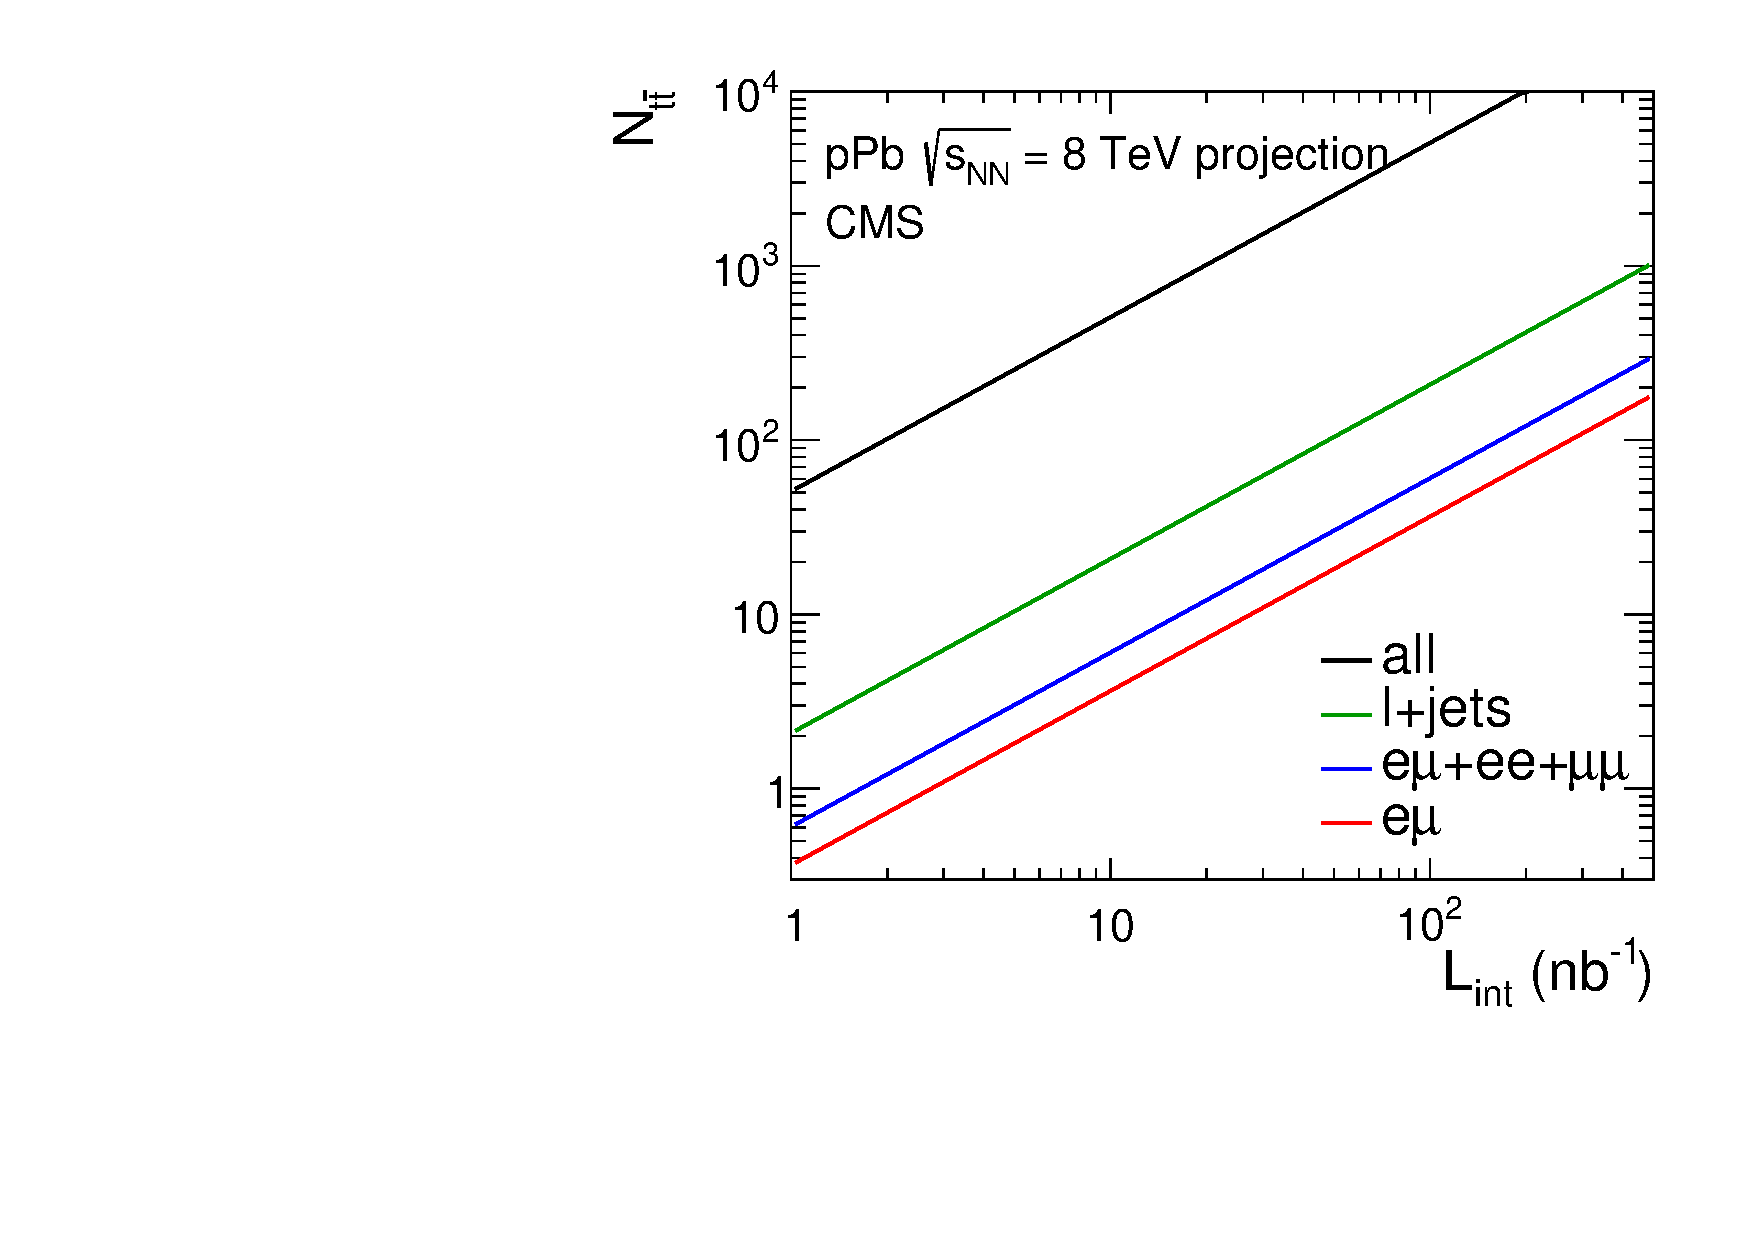
\includegraphics[width= 0.43\textwidth]{figures/top/ProjectedTTbarYield.pdf}
  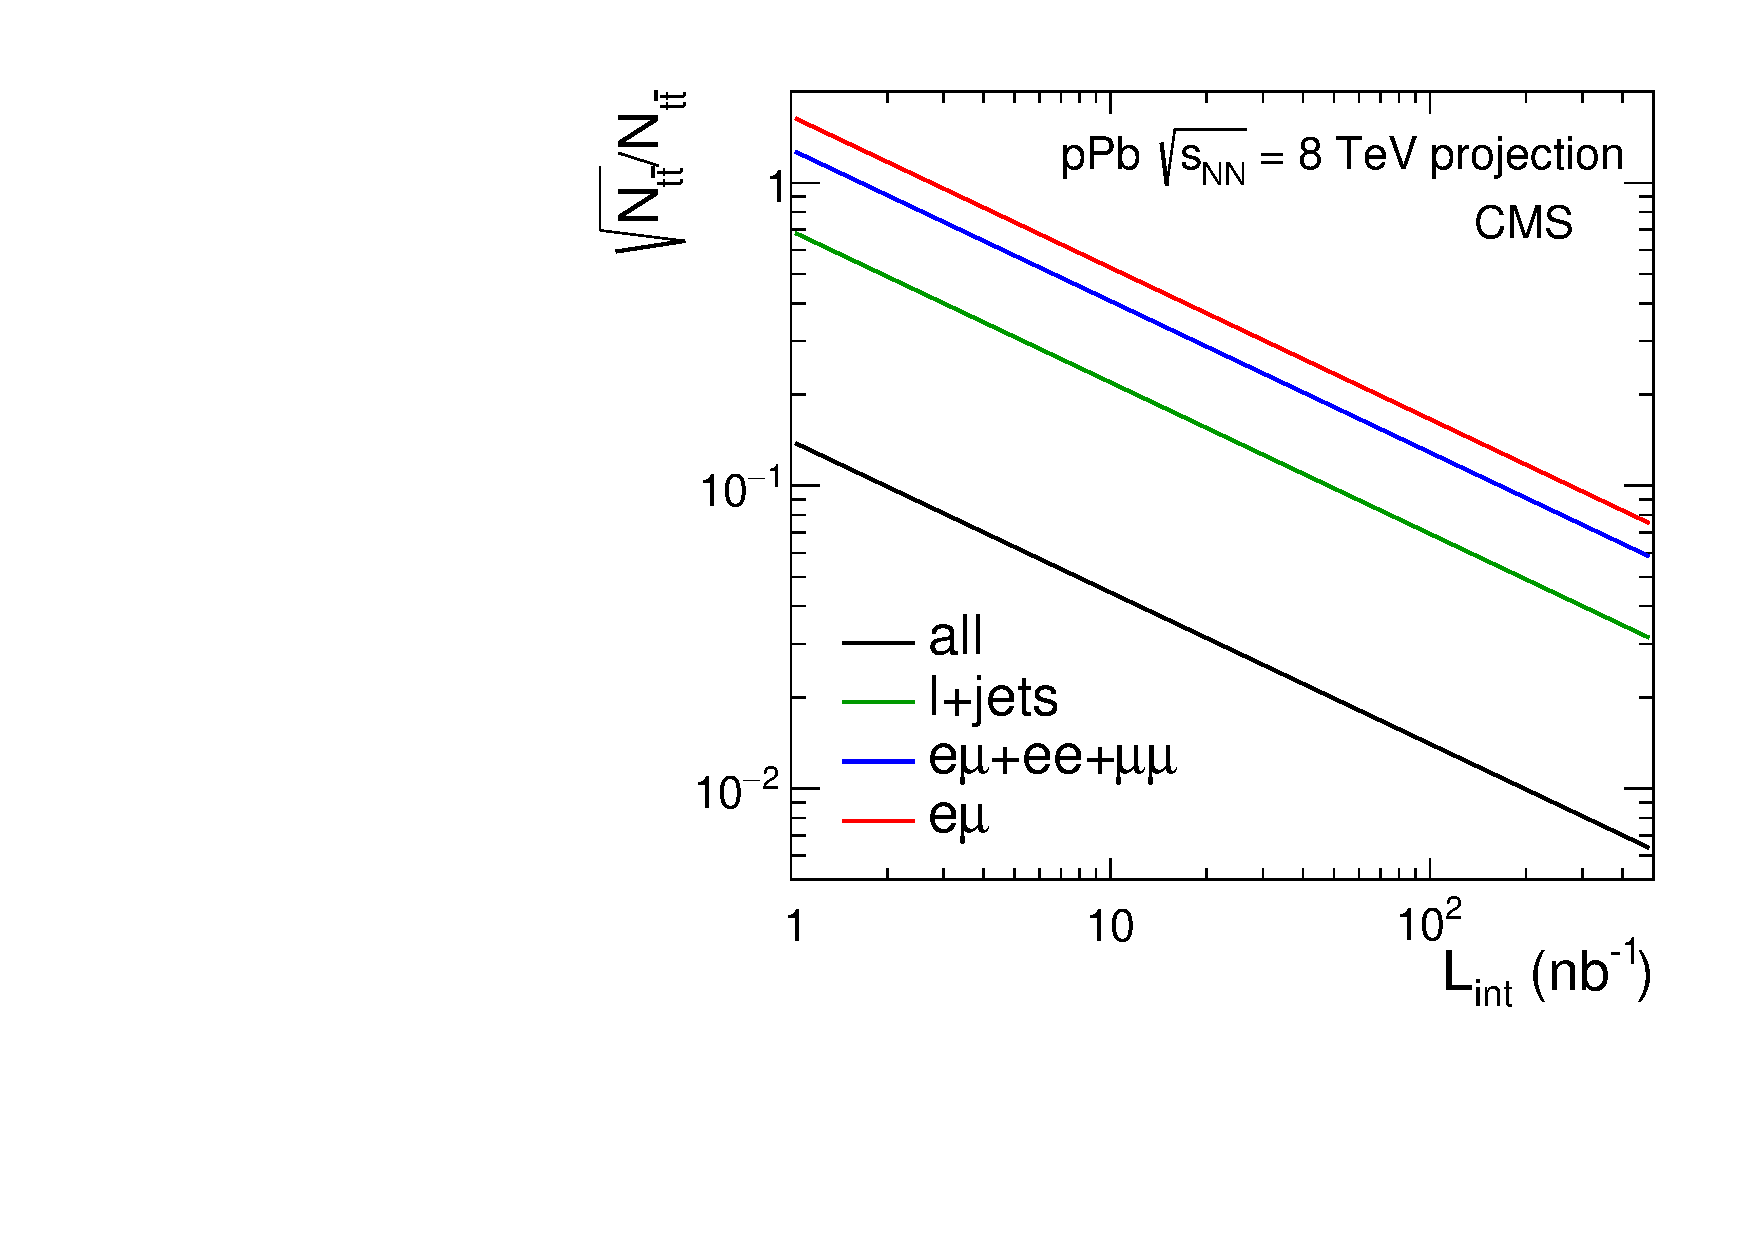
\includegraphics[width= 0.43\textwidth]{figures/top/ProjectedTTbarStatUnc.pdf}
  \caption{Left panel: Expected number of $\mathrm{t}\bar{\mathrm{t}}$ events for several channels in pPb collisions at $\sqrt{s_{\mathrm{NN}}}=8$ TeV as function of total integrated luminosity. Right panel: Corresponding statistical uncertainty as function of total integrated luminosity.
  }
\label{fig:ttPPbProjections}
\end{center}
\end{figure}

\begin{figure}[h!]
\begin{center}
  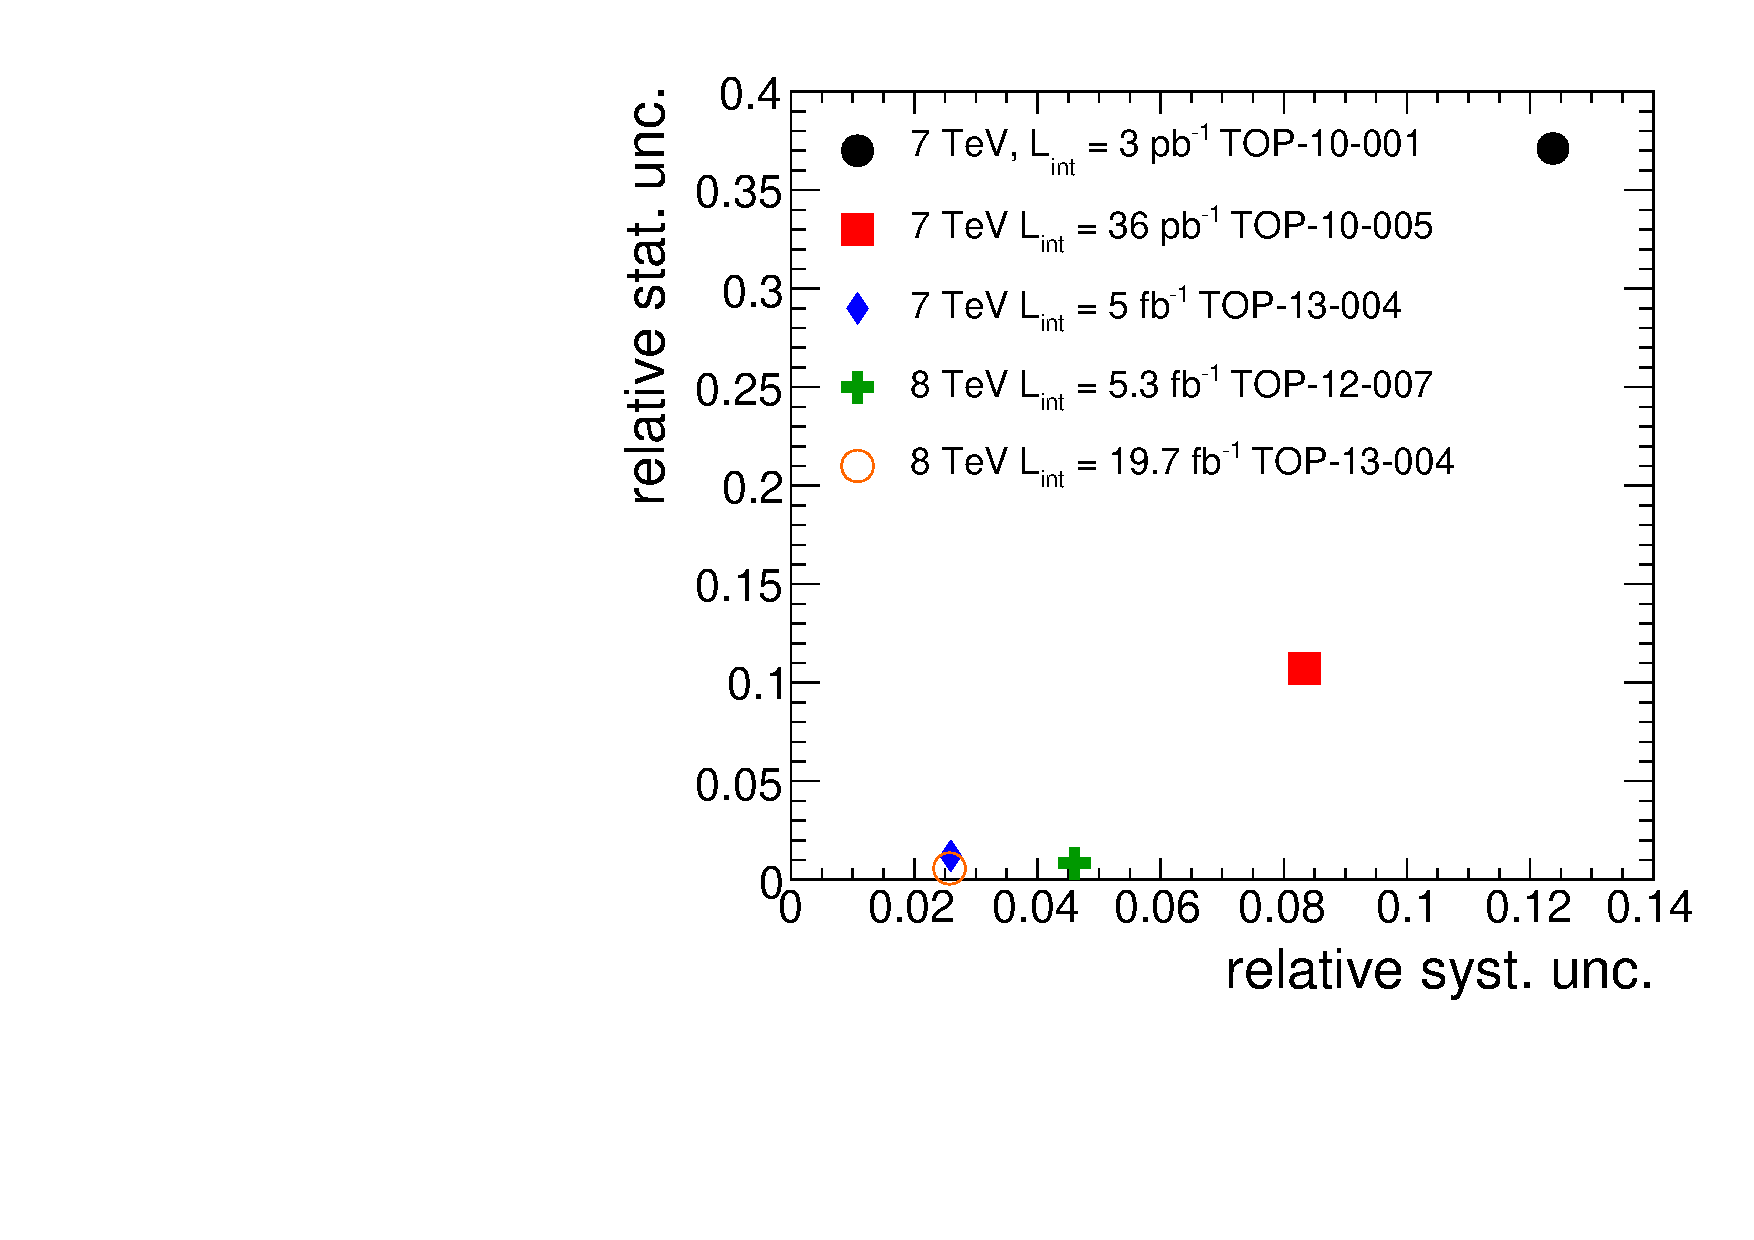
\includegraphics[width= 0.43\textwidth]{figures/top/topToLLXSecUncertaintiesPP.pdf}
  \caption{Evolution of statistical an systematic uncertainty of top pair cross section measurements in the fully leptonic channel in pp collisions at 7 and 8 TeV.
  }
\label{fig:ttStatSyst}
\end{center}
\end{figure}
